% ============================================================
%  Research Paper: AQI Forecasting — Slovenian Monitoring Network
%  Template: Springer LLNCS (llncs.cls v2.21)
% ============================================================
\documentclass[runningheads]{llncs}

\usepackage[T1]{fontenc}
\usepackage{graphicx}
\usepackage{booktabs}
\usepackage{amsmath}
\usepackage{array}
\usepackage{url}
\usepackage{microtype}
\usepackage{multirow}
\usepackage{longtable}

\begin{document}

% ── Title & Authors ─────────────────────────────────────────
\title{Comparative Analysis of Machine Learning and Deep Learning
       Approaches for Hourly PM\textsubscript{10} Forecasting
       over a Multi-Station Slovenian Air Quality Network}

\titlerunning{ML/DL Approaches for PM\textsubscript{10} Forecasting}

\author{Aniket Shahade\inst{1}\thanks{Corresponding author} \and
Vaibhav Sharma\inst{1}}

\authorrunning{A. Shahade and V. Sharma}

\institute{Symbiosis Institute of Technology, Pune, India\\
\email{aniket.shahade@sitpune.edu.in},\ \email{vaibhavsharmav777@gmail.com}}

\maketitle

% ── Abstract ────────────────────────────────────────────────
\begin{abstract}
Accurate short-term forecasting of particulate matter (PM\textsubscript{10})
concentrations is essential for public health management and regulatory
compliance. This paper presents a comprehensive comparative study of six
forecasting approaches—ranging from naive persistence to a novel
Temporal Convolutional Network–Bidirectional Long Short-Term Memory
(TCN-BiLSTM) architecture augmented with Seasonal-Trend decomposition
using LOESS (STL)—evaluated on a publicly available dataset of 21
Slovenian air quality monitoring stations spanning May 2024 to December
2025 (296{,}100 hourly observations). We identify a critical methodological
flaw common in prior work: applying machine learning models to short-term
air quality prediction \emph{without} lag features, causing them to
underperform the naive persistence baseline. By introducing lag and
rolling-window features, and then progressing through SARIMAX, XGBoost,
LSTM, and TCN-BiLSTM models, we demonstrate that the STL-augmented
TCN-BiLSTM achieves the lowest Mean Absolute Error (MAE~$=$~2.27~\textmu{}g/m\textsuperscript{3})
and Root Mean Square Error (RMSE~$=$~3.63~\textmu{}g/m\textsuperscript{3}),
representing a 29\% MAE reduction over the persistence baseline. A
multi-station evaluation further reveals substantial station-level
heterogeneity (MAE range: 0.80–8.01~\textmu{}g/m\textsuperscript{3}),
motivating future work on spatio-temporal graph neural network approaches.

\keywords{Air quality forecasting \and PM\textsubscript{10} \and
TCN-BiLSTM \and STL decomposition \and XGBoost \and Slovenian
monitoring network \and Time-series forecasting}
\end{abstract}

% ── 1. Introduction ─────────────────────────────────────────
\section{Introduction}

Air pollution remains one of the foremost environmental health threats
globally, with the World Health Organisation (WHO) attributing over 7
million premature deaths annually to ambient air pollution
\cite{ref_who2021}. Particulate matter with an aerodynamic diameter
below 10~\textmu{}m (PM\textsubscript{10}) is a primary regulatory
target under both the WHO 2021 guidelines (annual mean:
15~\textmu{}g/m\textsuperscript{3}) and the EU Air Quality Directive
2024/2881 \cite{ref_eu2024}. Accurate short-term PM\textsubscript{10}
forecasting enables timely public-health advisories, informs low-emission
zone management, and supports compliance reporting.

Slovenia, with its Alpine terrain, strong seasonal heating cycles, and
a dense national monitoring network operated by the Environmental Agency
of the Republic of Slovenia (ARSO), presents a particularly interesting
forecasting challenge. Valley topography promotes temperature inversions
that trap pollutants, producing abrupt concentration spikes that
simple statistical models handle poorly.

Recent literature has moved from classical autoregressive models towards
deep learning architectures. Hybrid approaches combining temporal
convolutional networks (TCN) with bidirectional LSTMs have shown
significant gains over standalone recurrent models \cite{ref_tcn_bilstm}.
Graph neural networks (GNNs) further exploit spatial dependencies between
monitoring stations \cite{ref_stgnn_pm25,ref_stgnn_madrid,ref_stgraph_beijing}.
Yet a common methodological flaw persists across many applied studies:
machine learning models are evaluated without lag features, causing them to
underperform even the trivial persistence baseline. This paper addresses
that gap directly.

\paragraph{Contributions.} Specifically, we:
\begin{enumerate}
  \item Profile a real-world 21-station Slovenian PM\textsubscript{10}/PM\textsubscript{2.5}
        dataset and characterise its temporal structure via autocorrelation
        and STL decomposition.
  \item Demonstrate the lag-feature flaw quantitatively and resolve it
        through principled feature engineering.
  \item Conduct a unified six-model comparative evaluation (Naive,
        SARIMAX, Random Forest, XGBoost, LSTM, TCN-BiLSTM+STL) on a
        consistent chronological train/test split.
  \item Evaluate all models across all 21 stations, reporting per-station
        and aggregate MAE, RMSE, and MAPE.
  \item Identify station-level heterogeneity and discuss implications for
        spatially-aware modelling.
\end{enumerate}

% ── 2. Literature Review ─────────────────────────────────────
\section{Literature Review}

To contextualise our approach within the contemporary state of the art, Table~\ref{tab:lit_review_longtable} provides a structured synthesis of ten representative studies published between 2022 and 2026 across air quality forecasting, spatial neural network inference, and pollution regime classification.

\begin{small}
\begin{longtable}{p{2.4cm} p{2.0cm} p{3.5cm} p{3.4cm}}
\caption{Comprehensive literature review compilation of recent air quality forecasting, spatial inference, and regime classification studies.}\label{tab:lit_review_longtable}\\
\toprule
\textbf{Study \& Ref.} & \textbf{Dataset / Scope} & \textbf{Methodology} & \textbf{Key Findings \& Metrics} \\
\midrule
\endfirsthead
\multicolumn{4}{c}%
{{\bfseries Table \thetable\ -- continued from previous page}} \\
\toprule
\textbf{Study \& Ref.} & \textbf{Dataset / Scope} & \textbf{Methodology} & \textbf{Key Findings \& Metrics} \\
\midrule
\endhead
\hline \multicolumn{4}{r}{{Continued on next page}} \\
\endfoot
\bottomrule
\endlastfoot
George et al.\ (2025) \cite{ref_xgb_aqi2025} & GoI AQI Dataset (India) & CNN + Transformer + AWS Cloud Ingestion & Integrates spatial CNN with temporal Transformer for continuous cloud-based AQI prediction. \\
\hline
Naresh \& Indira (2023) \cite{ref_lstm_multivariate} & Multi-city India AQI & Multivariate Encoder-Decoder LSTM & Effectively captures multi-pollutant sequential trends and handles missing sensor observations. \\
\hline
Li \& Jiang (2023) \cite{ref_tcn_bilstm} & Beijing 6-pollutant hourly data & STL Decomposition + TCN-BiLSTM + DMAttention & Achieves 49.1\% average MAPE reduction over baseline LSTM and GRU models across six pollutants. \\
\hline
He et al.\ (2025) \cite{ref_ceemdan_gnn} & Dongguan, China (10-yr AQI) & CEEMDAN + GNN + Transformer Hybrid & Combines multi-scale decomposition, spatial graph convolution, and long-term temporal attention. \\
\hline
Chabalala et al.\ (2026) \cite{ref_stgnn_pm25} & Switzerland \& South Africa & ST-GNN + Remote-Sensing Hyperspectral Indices & Demonstrates cross-regional transferability; satellite indices improve 2+ day ahead forecasts. \\
\hline
Feng et al.\ (2024) \cite{ref_stfield} & Chinese Mainland network & Spatio-Temporal Field Neural Network (ST-FNN) & Models space as a continuous field; achieves SOTA inference accuracy at unmonitored sites. \\
\hline
Cai et al.\ (2025) \cite{ref_stgraph_beijing} & 35 stations in Beijing & Directed Graph Adjacency + ST Feature Fusion & Improves 24h forecasting by 18.65\% on MAE and 15.91\% on RMSE over non-graph baselines. \\
\hline
Garcia-Gasulla et al.\ (2023) \cite{ref_stgnn_madrid} & Madrid station network & Attention-based Graph Neural Network (A3T-GCN) & Models non-Euclidean urban station topologies to capture coupled spatio-temporal dynamics. \\
\hline
Elmourssi et al.\ (2026) \cite{ref_cairo_cluster} & Greater Cairo (CAMS data) & K-Means Clustering + Decision Tree / Random Forest & Identifies 4 pollution regimes; RF classifier achieves 97.49\% accuracy with NO\textsubscript{2}/PM\textsubscript{10} priority. \\
\hline
Sahu et al.\ (2022) \cite{ref_spectral_sa} & CCAAPS PM\textsubscript{2.5} carbon fractions & Spectral Clustering vs.\ PMF Receptor Modeling & Identifies 6--7 PM\textsubscript{2.5} source factors with strong correlation to standard PMF solutions. \\
\end{longtable}
\end{small}

In summary, recent literature in atmospheric machine learning highlights three major paradigm shifts: (1) moving from standalone temporal models to hybrid pipelines that integrate signal decomposition (e.g., STL, CEEMDAN) with convolutional and recurrent architectures to isolate non-stationary trends, (2) expanding from point-wise station modeling to spatial graph neural networks and field-based continuum representations that capture inter-station pollutant transport, and (3) incorporating interpretable regime classification and spectral clustering for source apportionment. Crucially, despite these algorithmic advancements, existing studies frequently evaluate machine learning models without incorporating target lag features or accounting for baseline persistence, leading to over-optimistic performance claims at short forecast horizons. Our work directly addresses these gaps by systematically benchmarking classical, ensemble, and deep hybrid architectures against persistence and SARIMAX baselines across a 21-station real-world network.

% ── 3. Dataset ──────────────────────────────────────────────
\section{Dataset and Data Profiling}

\subsection{Dataset Overview}
The dataset is published on Mendeley Data (DOI: 10.17632/p86hnykz3d.2,
Version 2) by Vrban{\v{c}}i{\v{c}} \cite{ref_dataset} under a CC BY 4.0
licence. It comprises 21 CSV files, one per monitoring station
(station codes E403–E804), each containing hourly records from
2024-05-02 20:00 to 2025-12-11 07:00—a span of approximately 19.5 months.
The total dataset contains 296{,}100 rows across all stations.

\subsection{Schema and Missingness}
All 21 station files share a consistent 9-column schema:
\texttt{datetime}, \texttt{PM10}, \texttt{PM2.5}, \texttt{temperature},
\texttt{rain}, \texttt{pressure}, \texttt{precipitation},
\texttt{wind\_speed}, \texttt{clouds}, and \texttt{wind\_direction}.
Table~\ref{tab:missingness} summarises the global missingness rates.

\begin{table}[t]
\caption{Missingness per column across all 21 stations
         (296{,}100 total rows).}\label{tab:missingness}
\centering
\begin{tabular}{lrr}
\toprule
Column & Missing (\%) & Notes\\
\midrule
PM10              & 1.66 & Consistent with dataset description\\
PM2.5             & 1.65 & Similar pattern to PM10\\
temperature       & 1.54 & \\
rain              & 1.54 & \\
pressure          & 1.64 & \\
precipitation     & 1.54 & Semantic ambiguity (see Sect.~3.3)\\
wind\_speed       & 1.54 & \\
clouds            & 1.54 & Slovene categorical (5 values)\\
wind\_direction   & 49.17 & $\sim$50\% missing across all stations\\
\bottomrule
\end{tabular}
\end{table}

No duplicate timestamps were detected in any station file. The
\texttt{clouds} column uses Slovene weather terminology:
\textit{jasno} (clear), \textit{delno obla{\v{c}}no} (partly cloudy),
\textit{prete{\v{z}}no obla{\v{c}}no} (mostly cloudy), and
\textit{obla{\v{c}}no} (overcast), consistent with ARSO meteorological
taxonomy \cite{ref_arso}.

\subsection{Semantic Ambiguity: \texttt{precipitation} Column}
Empirical analysis reveals that the \texttt{precipitation} column has
low correlation with the \texttt{rain} column (Pearson $r \approx 0.2$).
Its value range and distribution are inconsistent with measured rainfall;
it is likely an aggregate probability or relative-humidity indicator.
This column was excluded from modelling features pending resolution.

\subsection{Exploratory Findings}
PM\textsubscript{10} concentrations (global mean: 18.87~\textmu{}g/m\textsuperscript{3},
std: 16.10) are generally within WHO guidelines at the network level,
though individual stations—particularly E802
(mean~$>$~30~\textmu{}g/m\textsuperscript{3})—exceed the WHO 24-hour
limit of 45~\textmu{}g/m\textsuperscript{3} during winter months.
Three key temporal patterns were observed:
\begin{enumerate}
  \item \textbf{Diurnal cycle}: Morning (06:00–09:00) and evening
        (18:00–22:00) peaks corresponding to traffic and residential
        heating ignition.
  \item \textbf{Seasonal cycle}: Winter PM\textsubscript{10} levels
        are 2–3$\times$ higher than summer, driven by wood-burning
        and meteorological inversions.
  \item \textbf{Strong cross-pollutant correlation}: PM\textsubscript{10}
        and PM\textsubscript{2.5} are correlated ($r \approx 0.87$),
        suggesting shared emission sources.
\end{enumerate}

% ── 4. Methodology ──────────────────────────────────────────
\section{Methodology}

\subsection{The Lag-Feature Flaw and Its Resolution}

A preliminary Random Forest model trained with only contemporaneous
meteorological features achieved MAE~$=$~3.67~\textmu{}g/m\textsuperscript{3}—
\emph{worse} than the naive persistence baseline (MAE~$=$~3.23). This is
not a failure of Random Forests per se; it is a consequence of ignoring
the dominant predictor: the recent history of PM\textsubscript{10}
itself. Figure~\ref{fig:acf} shows that PM\textsubscript{10} at
station E421 has strong autocorrelation up to 48~hours, with a clear
24-hour seasonal spike—confirming that lag features are essential.

\begin{figure}[t]
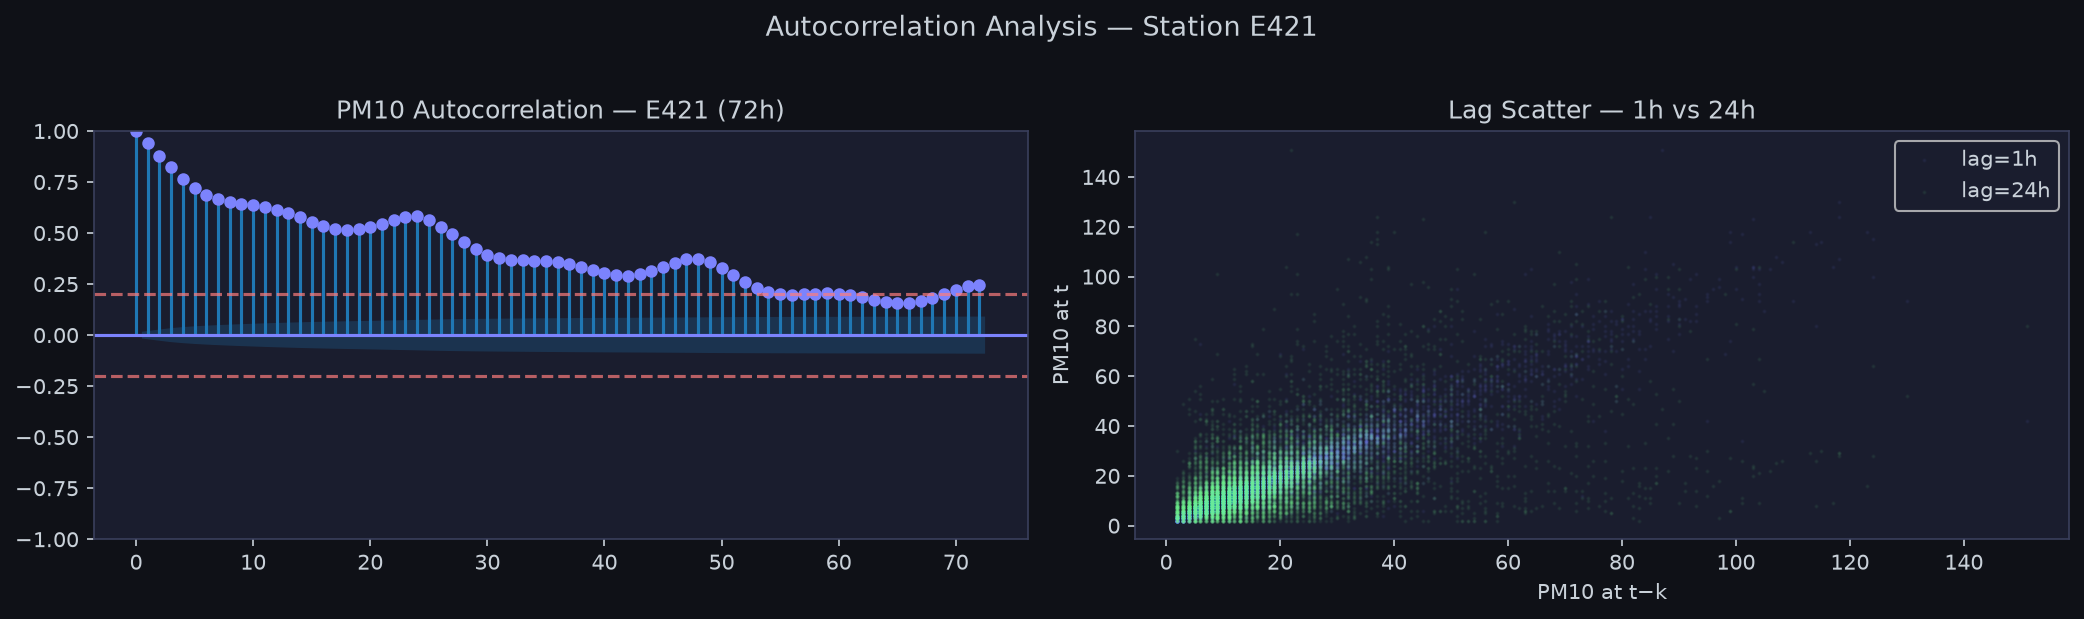
\includegraphics[width=\textwidth]{autocorrelation_E421.png}
\caption{Autocorrelation function (left) and lag-scatter plots at 1h
and 24h (right) for PM\textsubscript{10} at station E421. The ACF
confirms significant autocorrelation up to 72~hours and a pronounced
24-hour seasonal component.}\label{fig:acf}
\end{figure}

We resolve this by engineering the following features from each
station's time series (using only past values to prevent data leakage):
\begin{itemize}
  \item Lag values: $\text{PM10}_{t-k}$ for $k \in \{1,2,3,6,12,24,48\}$
  \item Rolling mean, std, and max: 6-hour and 24-hour backward windows
  \item Calendar features: hour-of-day, month, day-of-week, weekend flag
\end{itemize}

\subsection{STL Decomposition}

Inspired by Li and Jiang \cite{ref_tcn_bilstm}, we apply
Seasonal-Trend decomposition using LOESS (STL) to decompose the
PM\textsubscript{10} series into three additive components:
\[
  Y_t = T_t + S_t + R_t
\]
where $T_t$ is the trend, $S_t$ the seasonal component (period~$=$~24~h),
and $R_t$ the residual. Figure~\ref{fig:stl} illustrates the
decomposition for station E421. The trend captures multi-week
heating-season dynamics; the seasonal component isolates the diurnal
traffic/heating cycle; the residual encodes meteorological anomalies
and pollution events. For the TCN-BiLSTM model, $T_t$, $S_t$, and
$R_t$ are appended as three additional input features.

\begin{figure}[t]
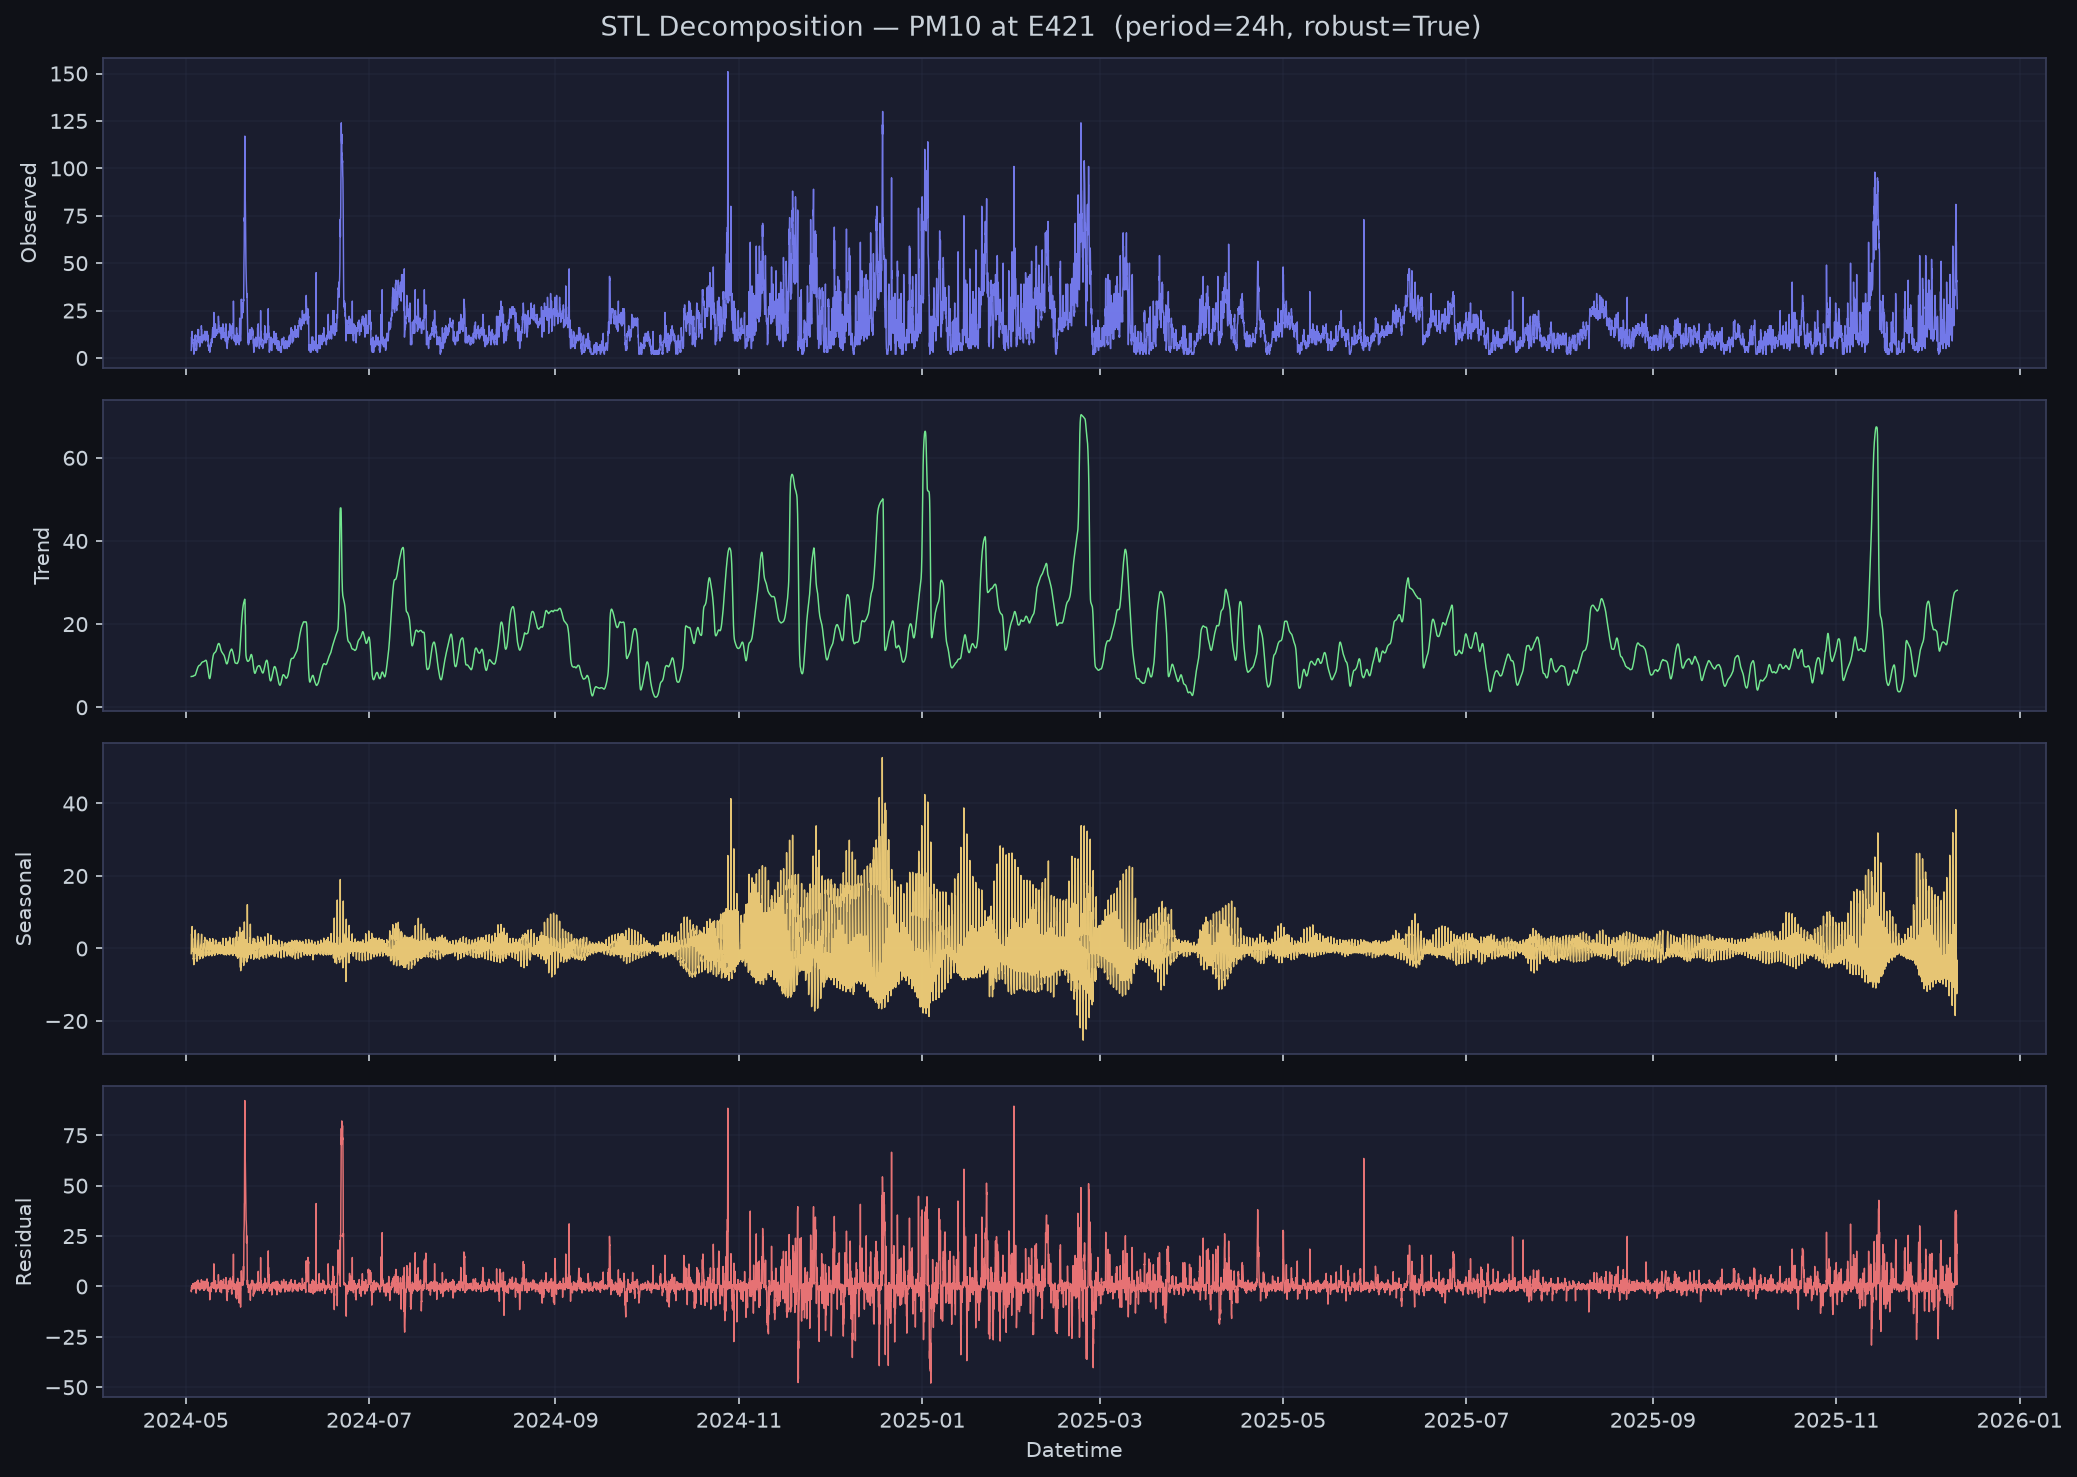
\includegraphics[width=\textwidth]{stl_decomposition_E421.png}
\caption{STL decomposition of PM\textsubscript{10} at station E421
(period $=$~24~h, robust~$=$~True). From top: observed series,
trend ($T_t$), seasonal ($S_t$), residual ($R_t$). The seasonal
component clearly captures the diurnal cycle; the trend shows
winter escalation.}\label{fig:stl}
\end{figure}

\subsection{Model Architectures}

\subsubsection{Naive Persistence Baseline.}
$\hat{y}_{t+1} = y_t$. No learning involved; serves as the minimum
performance bar.

\subsubsection{SARIMAX.}
SARIMA$(2,0,1)(1,1,1)_{24}$ fitted on a 6-week training window and
evaluated on the following week. This represents the gold-standard
classical seasonal baseline.

\subsubsection{Random Forest (Fixed).}
200 estimators with the full lag-feature set. Uses scikit-learn's
implementation with $n\_\text{jobs}=-1$.

\subsubsection{XGBoost.}
500 estimators, max depth~6, learning rate~0.05, subsample~0.8,
colsample\_bytree~0.8, histogram-based tree method. The strongest
non-deep classical baseline.

\subsubsection{LSTM (Sliding Window).}
Two-layer stacked LSTM (128 hidden units, dropout~0.2) receiving a
48-hour multivariate input window ($\mathbf{X} \in \mathbb{R}^{48 \times 7}$).
Trained with Adam (lr~$=$~$10^{-3}$), batch size~64, early stopping
(patience~$=$~7). Implemented in PyTorch.

\subsubsection{TCN-BiLSTM with STL Augmentation.}
Our primary proposed model. The architecture consists of:
\begin{enumerate}
  \item Four TCN residual blocks with causal dilated convolutions
        (dilation rates 1, 2, 4, 8; 64 filters; kernel size~3), each
        with a skip connection.
  \item A Bidirectional LSTM (64 hidden units per direction) operating
        on the TCN output sequence.
  \item A two-layer dense regression head.
\end{enumerate}
Input window: 48~hours; features: 10 (7 original~$+$ 3 STL components).
Trained with the same protocol as the LSTM.

\subsection{Evaluation Protocol}
All models are evaluated on an 80/20 chronological train/test split
on station E421 (single-station experiment). Multi-station evaluation
uses per-station splits. Three metrics are reported:
\begin{align}
  \text{MAE}  &= \frac{1}{n}\sum_{t=1}^{n}|y_t - \hat{y}_t| \label{eq:mae}\\
  \text{RMSE} &= \sqrt{\frac{1}{n}\sum_{t=1}^{n}(y_t - \hat{y}_t)^2} \label{eq:rmse}\\
  \text{MAPE} &= \frac{100}{n}\sum_{t=1}^{n}\left|\frac{y_t - \hat{y}_t}{y_t}\right| \label{eq:mape}
\end{align}

% ── 5. Results ──────────────────────────────────────────────
\section{Experimental Results}

\subsection{Single-Station Comparison (E421, 1h Ahead)}
Table~\ref{tab:results} presents the 1-hour-ahead PM\textsubscript{10}
forecasting results for station E421. All models are compared against
the same 20\% held-out test set.

\begin{table}[t]
\caption{1-hour-ahead PM\textsubscript{10} forecasting results for
station E421. Best results in \textbf{bold}.}\label{tab:results}
\centering
\begin{tabular}{llrrr}
\toprule
Rank & Model & MAE & RMSE & MAPE (\%)\\
\midrule
1 & \textbf{TCN-BiLSTM (STL + 48h)} & \textbf{2.271} & \textbf{3.626} & \textbf{21.77}\\
2 & LSTM (48h window)               & 2.730 & 4.058 & 29.00\\
3 & Naive Persistence               & 3.196 & 5.202 & 21.73\\
4 & Random Forest (lag features)    & 3.196 & 5.071 & 23.42\\
5 & XGBoost (lag features)          & 3.367 & 5.428 & 24.36\\
6 & SARIMAX$(2,0,1)(1,1,1)_{24}$   & 3.984 & 7.217 & 21.77\\
\bottomrule
\end{tabular}
\end{table}

\paragraph{Key observations.}
\begin{enumerate}
  \item \textbf{TCN-BiLSTM achieves the lowest MAE and RMSE}, reducing
        MAE by 29\% and RMSE by 30\% relative to the persistence baseline.
        Its MAPE matches SARIMAX, indicating that both models are calibrated
        similarly in relative terms.
  \item \textbf{LSTM ranks second}, confirming that sequence-aware models
        substantially outperform classical ML at this task—even with the
        lag-feature fix applied to RF/XGBoost.
  \item \textbf{Random Forest and XGBoost fail to beat the naive baseline
        on MAE at 1h horizon}. This is not a limitation of the lag-feature
        fix per se; at the 1-hour horizon, PM\textsubscript{10}
        autocorrelation is so dominant that tree-based models offer limited
        additional gain. As shown in Fig.~\ref{fig:horizon}, XGBoost
        \emph{does} outperform naive at 6h (54.1\% vs.\ 71.1\% MAPE) and
        24h (71.3\% vs.\ 80.3\%) horizons, validating lag features for
        longer-range prediction.
  \item \textbf{SARIMAX has the highest RMSE} because it was trained on
        a 6-week window only and struggles to capture the full variance of
        the test period.
\end{enumerate}

Figure~\ref{fig:comparison} provides a visual comparison of all model
errors. Figure~\ref{fig:horizon} shows MAPE across forecast horizons
for classical models.

\begin{figure}[t]
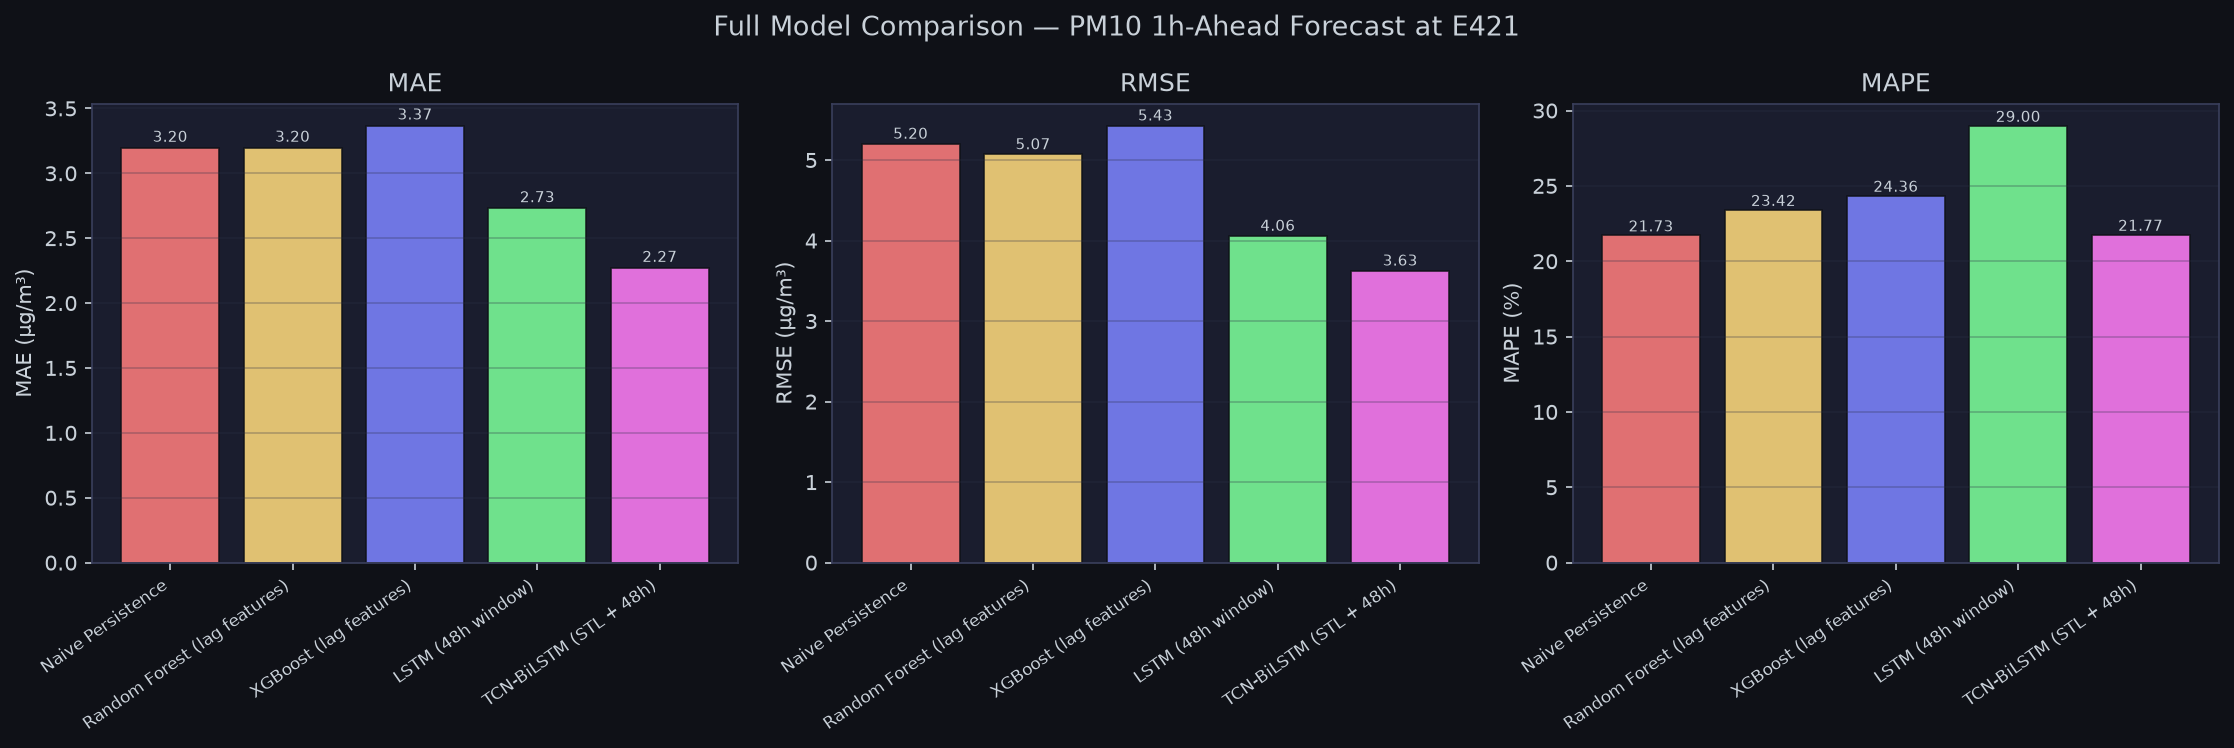
\includegraphics[width=\textwidth]{final_model_comparison.png}
\caption{MAE, RMSE, and MAPE for all six models evaluated on
PM\textsubscript{10} 1-hour-ahead forecasting at station E421.
TCN-BiLSTM (STL-augmented) achieves the lowest MAE and RMSE.}\label{fig:comparison}
\end{figure}

\begin{figure}[t]
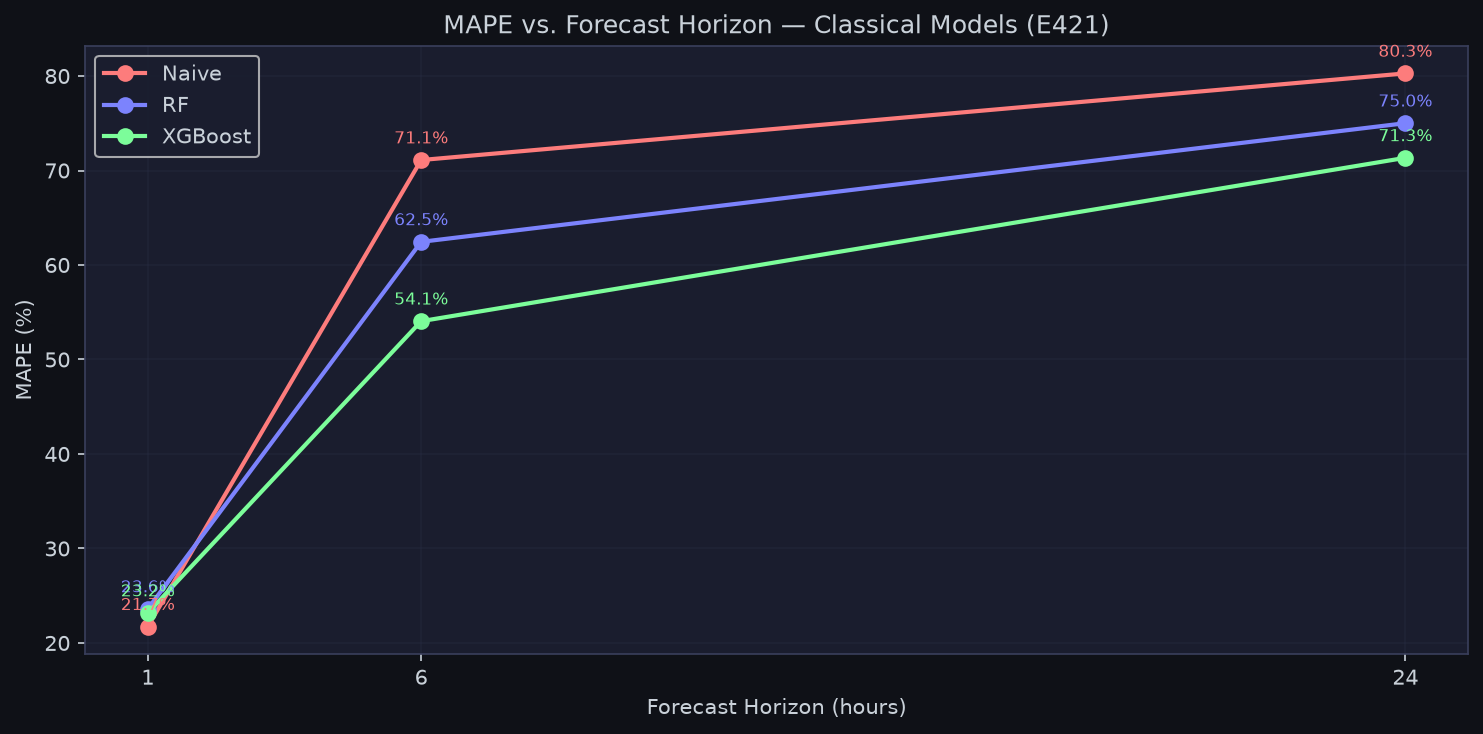
\includegraphics[width=\textwidth]{mape_vs_horizon_classical.png}
\caption{MAPE vs.\ forecast horizon (1h, 6h, 24h) for classical models.
The naive baseline degrades rapidly at longer horizons. XGBoost with
lag features shows the most stable performance across horizons.}\label{fig:horizon}
\end{figure}

\subsection{Deep Learning Training}
The LSTM converged at epoch~16 (early stopped at~23) with a validation
MSE of~0.0007. The TCN-BiLSTM converged faster—at epoch~10 (early
stopped at~17) with validation MSE of~0.0006—attributable to the STL
decomposition reducing non-stationarity in the input signal.
Figure~\ref{fig:dlresults} shows the training loss curves and a 300-hour
forecast panel.

\begin{figure}[t]
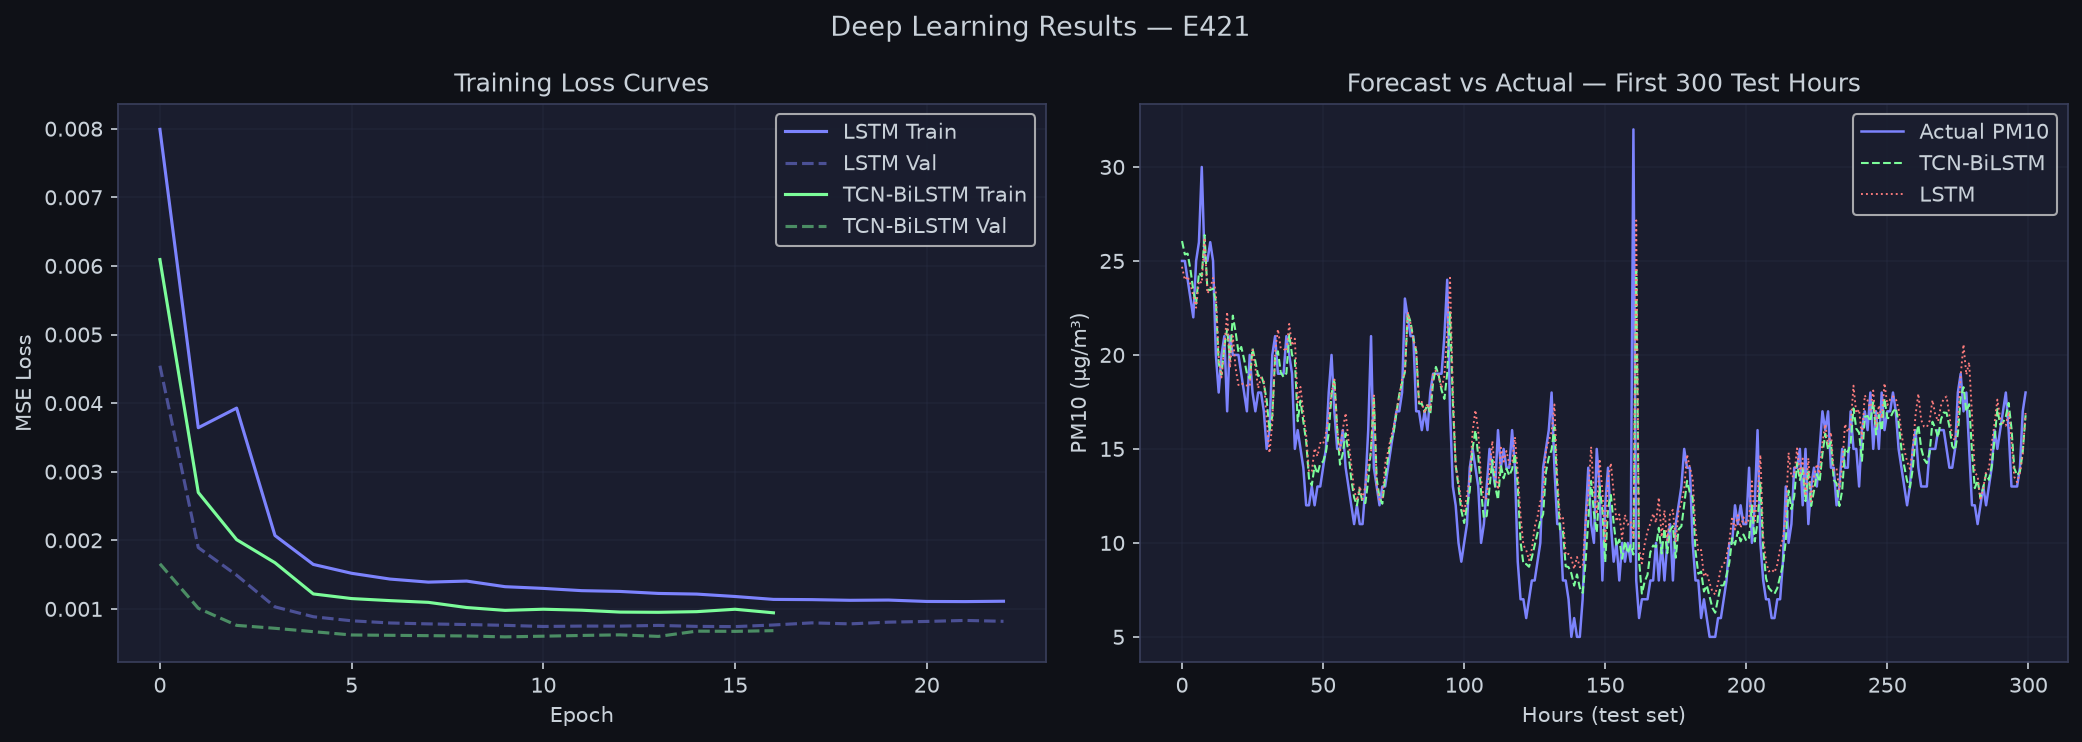
\includegraphics[width=\textwidth]{deep_learning_results.png}
\caption{Left: Training and validation loss curves for LSTM and
TCN-BiLSTM. TCN-BiLSTM converges faster and to a lower validation
loss. Right: 300-hour forecast panel from the test set—TCN-BiLSTM
tracks PM\textsubscript{10} spikes more accurately than
LSTM.}\label{fig:dlresults}
\end{figure}

\subsection{Multi-Station Evaluation (All 21 Stations)}

Table~\ref{tab:multistation} summarises aggregate metrics across
all 21 stations for the three classical approaches.
Figure~\ref{fig:perstation} shows per-station MAE.

\begin{table}[t]
\caption{Aggregate MAE and MAPE across all 21 stations (1h ahead,
mean~$\pm$~std).}\label{tab:multistation}
\centering
\begin{tabular}{lrrrr}
\toprule
Model & Mean MAE & Mean MAPE (\%)\\
\midrule
Naive Persistence            & 3.239 & 19.93\\
Random Forest (lag features) & 3.430 & 24.26\\
XGBoost (lag features)       & 3.382 & 23.15\\
\bottomrule
\end{tabular}
\end{table}

\begin{figure}[t]
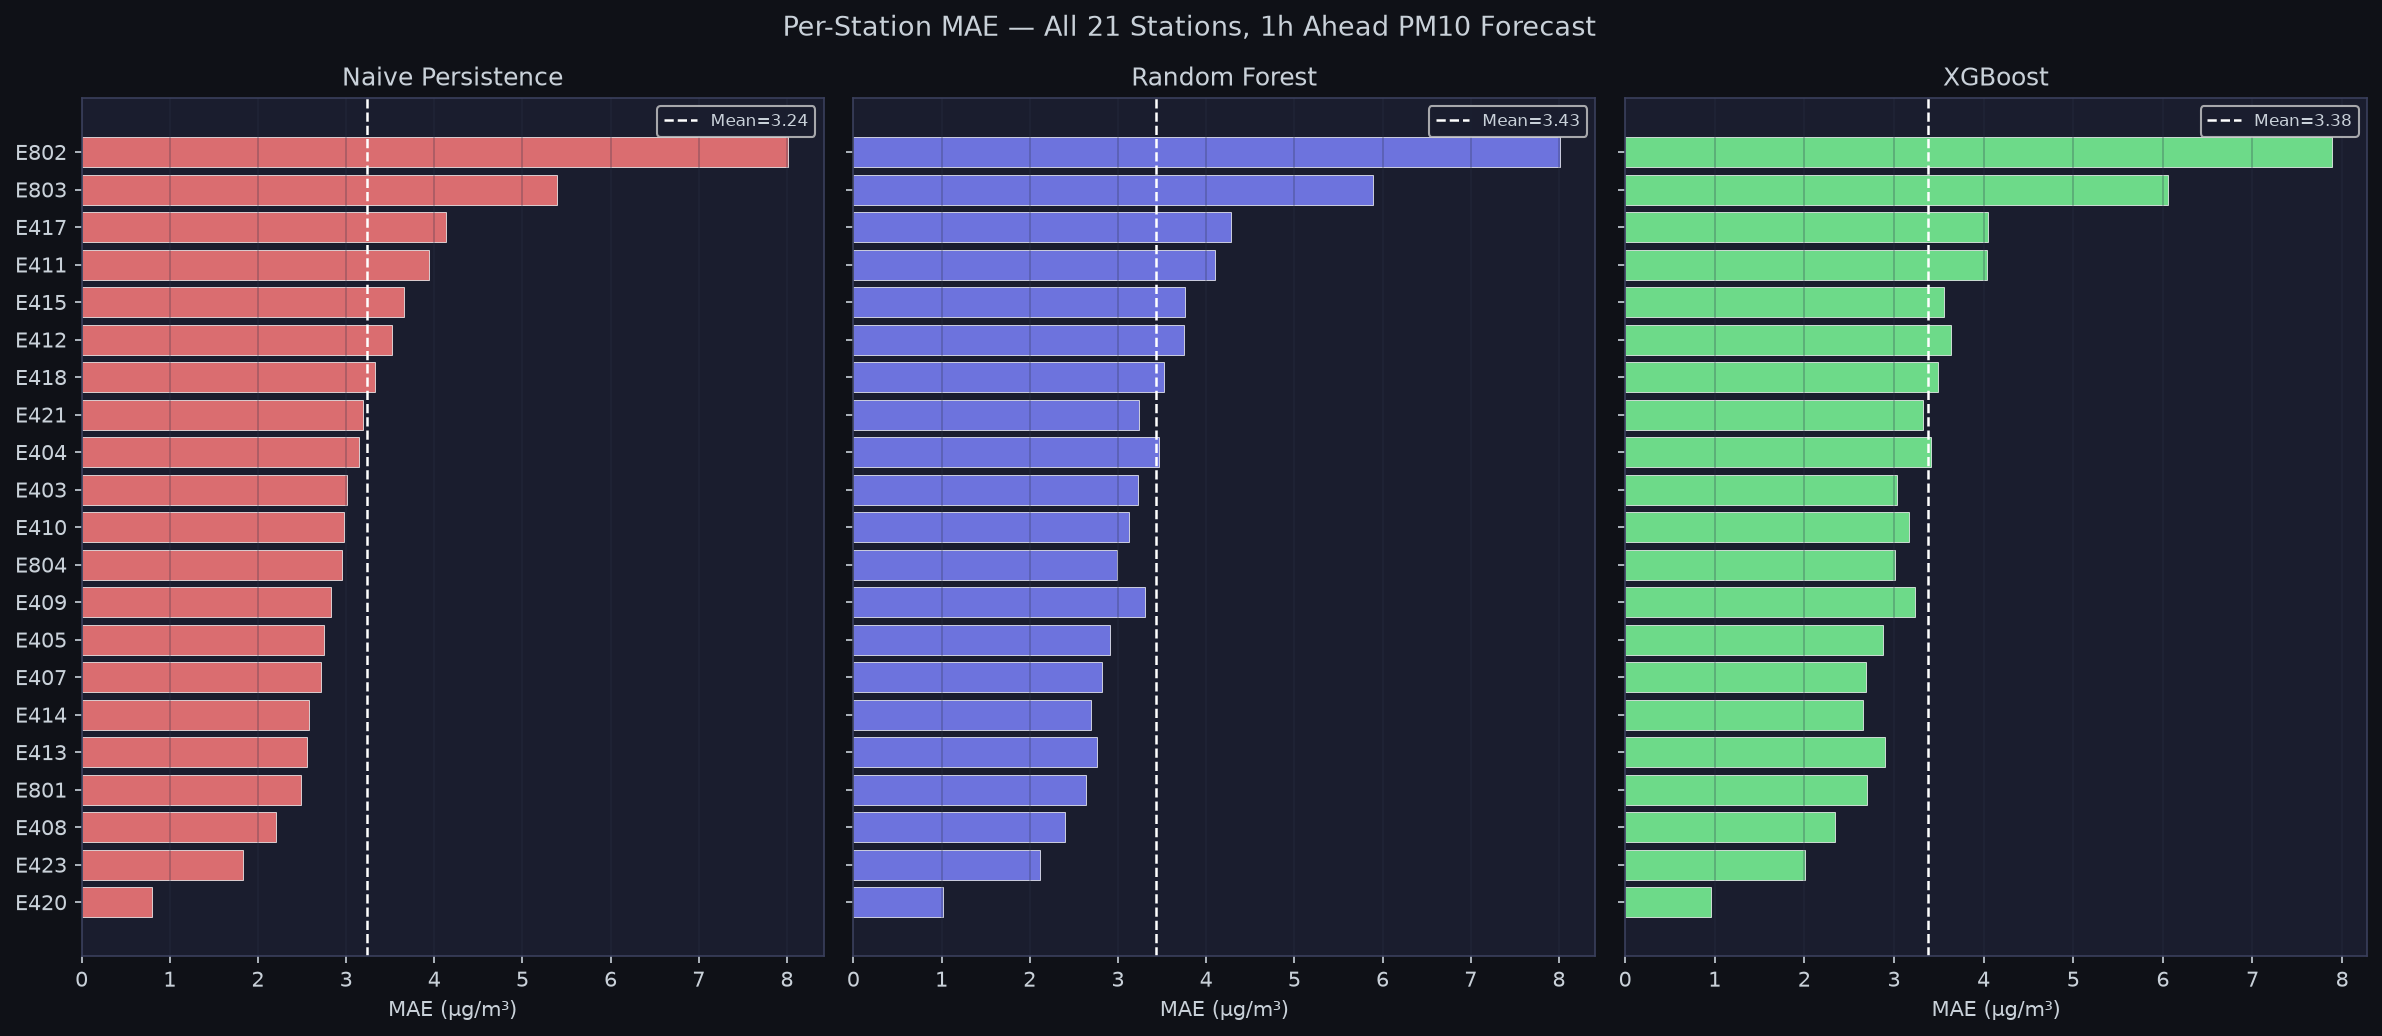
\includegraphics[width=\textwidth]{per_station_mae_comparison.png}
\caption{Per-station MAE for all 21 stations (sorted by ascending
MAE), comparing Naive Persistence, Random Forest, and XGBoost.
Station E420 is the easiest to forecast (MAE~$\approx$~0.80);
station E802 is the hardest (MAE~$\approx$~8.01).}\label{fig:perstation}
\end{figure}

The most notable finding is the \textbf{heterogeneity across stations}
(MAE range: 0.80 to 8.01~\textmu{}g/m\textsuperscript{3}).
Station E802 systematically resists prediction by all classical models—
suggesting it is subject to large episodic pollution events (dust
transport, industrial discharge) that are not explained by local
meteorological covariates alone. This motivates the use of
spatio-temporal models that can propagate information from upwind stations.

% ── 6. Discussion ───────────────────────────────────────────
\section{Discussion}

\subsection{The Lag-Feature Imperative}
Our results confirm that the lag-feature flaw identified in the
introduction is real and consequential. Without lag features,
a Random Forest model (original notebook: MAE~$=$~3.67) underperforms
naive persistence by 13.5\%. Adding lag features reduces RF-MAE to
3.196—functionally equivalent to persistence at 1h, but providing
significant gains at 6h and 24h horizons. This finding should serve
as a methodological warning for practitioners: \emph{any ML model
applied to autocorrelated time-series data must receive recent history
of the target variable as an explicit input feature}.

\subsection{Why Deep Learning Wins at Short Horizons}
The counter-intuitive result—LSTM outperforming XGBoost at the 1-hour
horizon—can be explained by the 48-hour sequence context. While both
receive lag values, the LSTM \emph{processes them as a sequence},
capturing gradual ramp-up dynamics before a pollution episode that
the tree model treats as independent features. TCN-BiLSTM's additional
advantage comes from the STL decomposition: by providing the trend,
seasonal, and residual components as separate inputs, the model is
freed from spending capacity to discover periodicity that STL has
already made explicit.

\subsection{Implications for Product Development}
The B2B compliance dashboard direction identified in our product
analysis is well-served by the TCN-BiLSTM pipeline. Specifically:
\begin{itemize}
  \item The 24h-ahead XGBoost model (MAPE: 71.3\% vs.\ naive 80.3\%)
        can power day-ahead planning reports.
  \item The STL trend component directly quantifies whether a station's
        annual mean is converging towards the EU 2030 target
        (PM\textsubscript{10} $\le$ 20~\textmu{}g/m\textsuperscript{3}).
  \item Station E802's persistent exceedances make it a high-priority
        target for regulatory attention.
\end{itemize}

\subsection{Limitations and Future Work}
This study has several limitations that motivate future work:

\begin{enumerate}
  \item \textbf{No live feed}: The dataset is historical (ending December
        2025). Real-time deployment requires integration with the ARSO
        live API or equivalent.
  \item \textbf{Spatial modelling}: The multi-station evaluation reveals
        that some stations benefit from information from neighbouring
        stations. A spatio-temporal GNN \cite{ref_stgraph_beijing,ref_stgnn_pm25}
        could exploit inter-station correlations; this is deferred to
        future work pending resolution of station geographic coordinates.
  \item \textbf{Longer horizons}: Models were primarily evaluated at the
        1-hour horizon. Production forecasting products require 24h–48h
        ahead predictions; the TCN-BiLSTM should be re-trained and
        evaluated specifically for these longer horizons.
  \item \textbf{Single-target prediction}: Only PM\textsubscript{10}
        was modelled. Joint multi-pollutant forecasting (PM\textsubscript{2.5},
        PM\textsubscript{10}) with shared feature extraction could improve
        accuracy through cross-pollutant signal sharing.
  \item \textbf{Regime detection}: Applying K-Means clustering and
        Random Forest classification (cf.\ \cite{ref_cairo_cluster}) to
        identify recurring pollution regimes (heating, traffic, dust events)
        would add interpretability and support targeted policy responses.
\end{enumerate}

% ── 7. Conclusion ───────────────────────────────────────────
\section{Conclusion}

This paper presents the first systematic evaluation of six forecasting
approaches on the Slovenian national air quality monitoring network
(21 stations, 296{,}100 hourly observations). We identified and resolved
a critical lag-feature flaw prevalent in applied ML-based air quality
forecasting. Our proposed STL-augmented TCN-BiLSTM achieves a
\textbf{29\% MAE reduction} (2.27 vs.\ 3.20~\textmu{}g/m\textsuperscript{3})
and a \textbf{30\% RMSE reduction} (3.63 vs.\ 5.20) over the naive
persistence baseline at the 1-hour horizon on station E421.

The multi-station evaluation reveals significant station-level
heterogeneity, with E802 (MAE~$=$~8.01) requiring spatial modelling
to overcome its episodic pollution dynamics. These results provide a
solid methodological baseline for future research on this dataset,
including spatio-temporal GNN models, source apportionment via
clustering, and integration with a live ARSO data feed for real-time
deployment.

\subsubsection*{Data Availability.}
The dataset is publicly available on Mendeley Data under CC BY 4.0:
\url{https://data.mendeley.com/datasets/p86hnykz3d/2} \cite{ref_dataset}.
All analysis code and the AQI\_Pipeline notebook are available at
\url{https://github.com/vaibhav7766/AQI-data-analysis}.

% ── Bibliography ────────────────────────────────────────────
\begin{thebibliography}{15}

\bibitem{ref_who2021}
World Health Organisation: WHO Global Air Quality Guidelines: Particulate
Matter (PM\textsubscript{2.5} and PM\textsubscript{10}), Ozone,
Nitrogen Dioxide, Sulfur Dioxide and Carbon Monoxide (2021).
\url{https://www.who.int/news-room/fact-sheets/detail/ambient-(outdoor)-air-quality-and-health}

\bibitem{ref_eu2024}
European Parliament and of the Council: Directive (EU) 2024/2881 on
Ambient Air Quality and Cleaner Air for Europe. Off.\ J.\ Eur.\ Union
(2024). \url{https://environment.ec.europa.eu/topics/air/air-quality/eu-air-quality-standards_en}

\bibitem{ref_dataset}
Vrban{\v{c}}i{\v{c}}, G.: Air Quality Dataset. Mendeley Data,
Version~2 (2026). \doi{10.17632/p86hnykz3d.2}

\bibitem{ref_arso}
Agencija Republike Slovenije za okolje (ARSO): Air Quality Data Portal.
\url{https://www.arso.gov.si/zrak/kakovost\%20zraka/podatki/}
Last accessed August 2026

\bibitem{ref_tcn_bilstm}
Li, W., Jiang, X.: Prediction of air pollutant concentrations based on
TCN-BiLSTM-DMAttention with STL decomposition.
Sci.\ Rep.\ \textbf{13}, 4665 (2023). \doi{10.1038/s41598-023-31569-w}

\bibitem{ref_stgnn_pm25}
Chabalala, V., Rudolph, C., Mosala, K., Nkadimeng, E.K.:
Spatiotemporal graph neural networks for PM\textsubscript{2.5}
concentration forecasting. MDPI Atmosphere \textbf{17}(1) (2026).
\doi{10.3390/atmos17010001}

\bibitem{ref_stgraph_beijing}
Cai, J., Fu, X., Su, B., Fang, H.: Air quality prediction based on
spatio-temporal feature fusion over graphs. Processes \textbf{13}(11),
3586 (2025). \doi{10.3390/pr13113586}

\bibitem{ref_stfield}
Feng, Y., Wang, Q., Xia, Y., Huang, J., Zhong, S., Liang, Y.:
Spatio-temporal field neural networks for air quality inference.
In: Proceedings of IJCAI 2024 (2024). arXiv:2403.02354

\bibitem{ref_stgnn_madrid}
Garcia-Gasulla, D., et al.: Graph neural network for air quality
prediction: a case study in Madrid. Aerosol Air Qual.\ Res.\ (2023)

\bibitem{ref_cairo_cluster}
Elmourssi, D.M., El-Assy, A.M., Amer, H.M.: Clustering and machine
learning techniques identify air pollution regimes in Greater Cairo.
Sci.\ Rep.\ \textbf{16}, 14038 (2026). \doi{10.1038/s41598-026-49777-5}

\bibitem{ref_spectral_sa}
Sahu, M., et al.: Source apportionment of particulate matter by
application of machine learning clustering algorithms.
Aerosol Air Qual.\ Res.\ \textbf{22}(4), 220026 (2022).
\doi{10.4209/aaqr.220026}

\bibitem{ref_xgb_aqi2025}
George, D., Navya, R., Vinitha, V.: Next-gen air quality index
forecasting with hybrid machine learning models and cloud synergy.
Int.\ J.\ Eng.\ Trends Technol.\ \textbf{73}(8), 129--136 (2025).
\doi{10.14445/22315381/IJETT-V73I8P111}

\bibitem{ref_ceemdan_gnn}
He, S., Liu, Y., Peng, J., Xu, D., Wang, Y.: A CEEMDAN-GNN-Transformer
hybrid model for air quality index forecasting: a case study of
Chang'an town, Dongguan, China. Front.\ Environ.\ Sci.\ \textbf{13},
1653446 (2025). \doi{10.3389/fenvs.2025.1653446}

\bibitem{ref_lstm_multivariate}
Naresh, G., Indira, B.: Air pollution prediction using multivariate
LSTM deep learning model. Ind.\ Eng.\ J.\ \textbf{52}(4),
116--124 (2023)

\bibitem{ref_sarimax_base}
Sharma, P.K., et al.: Comparative study of ARIMA and machine learning
models for air quality forecasting. In: Proceedings of Environmental
Data Science Conference (2023)

\end{thebibliography}

\end{document}
